\documentclass[a4paper,12pt]{article}

\usepackage[utf8]{inputenc}
\usepackage[T1]{fontenc}
\usepackage[frenchb]{babel}
\usepackage{a4wide}
\usepackage{graphicx}
\usepackage{subfig}
\usepackage{tikz}
\usepackage{ifthen}
\usepackage{ifpdf}
\usepackage{comment}
\usepackage{listings} % pour code XML
\usepackage[babel=true]{csquotes}


\graphicspath{{images/}}

\newlength\figureheight
\newlength\figurewidth

\ifpdf
\usepackage[pdftex]{hyperref}
\else
\usepackage{hyperref}
\fi

\usepackage{color}
\hypersetup{
colorlinks=true,
linkcolor=black,
citecolor=black,
urlcolor=black}

\renewcommand{\baselinestretch}{1.05}
\usepackage{fancyhdr}
\pagestyle{fancy}
\fancyfoot{}
\fancyhead[LE,RO]{\bfseries\thepage}
\fancyhead[RE]{\bfseries\nouppercase{\leftmark}}
\fancyhead[LO]{\bfseries\nouppercase{\rightmark}}
\setlength{\headheight}{15pt}

\let\headruleORIG\headrule
\renewcommand{\headrule}{\color{black} \headruleORIG}
\renewcommand{\headrulewidth}{1.0pt}
\usepackage{colortbl}
\arrayrulecolor{black}

\fancypagestyle{plain}{
  \fancyhead{}
  \fancyfoot[C]{\thepage}
  \renewcommand{\headrulewidth}{0pt}
}

\makeatletter
\def\cleardoublepage{\clearpage\if@twoside \ifodd\c@page\else
  \hbox{}
  \thispagestyle{empty}
  \newpage
  \if@twocolumn\hbox{}\newpage\fi\fi\fi}
\makeatother

\parskip=5pt

\usepackage{amsthm}
\usepackage{array}
\usepackage{bm}

\lstset{ % encadrer et coloriser un document XML
  language=xml,frame=single, 
  breaklines=true, 
  basicstyle=\ttfamily,
  basicstyle=\scriptsize, 
  keywordstyle=\color{blue}, 
  commentstyle=\color{green}, 
  stringstyle=\color{red}, 
  identifierstyle=\color{blue}
}



\begin{document}

%%%%%%%%%%%%%%%%%%%%%%%%%%%%%%%%%%%%%%%%%%%%  page de garde  %%%%%%%%%%%%%%%%%%

\begin{titlepage}
\begin{center}

\begin{minipage}[c]{.46\linewidth}
  \centering
  
\includegraphics[width=0.6\textwidth]{logo_UPMC.png}\\[1cm]
\end{minipage}
\hfill
\begin{minipage}[c]{.46\linewidth}
  \centering
  
\includegraphics[width=0.5\textwidth]{logo_ircam.png}\\[1cm]
\end{minipage}

\vspace*{1cm}

{\large Université Pierre et Marie Curie}\\[1cm]

{\large Master Informatique, Spécialité STL}\\[1cm]

{\large Semestre 2, UE Projet STL}\\[1cm]

% titre
\rule{\linewidth}{0.5mm} \\[0.5cm]
{ \huge \bfseries Un analyseur syntaxique pour MusicXML \\[0.4cm] }
\rule{\linewidth}{0.5mm} \\[0.5cm]

\vspace*{1cm}

% Auteurs
\noindent
\begin{minipage}{0.5\textwidth}
  \begin{flushleft} \large
    \emph{Auteurs :}\\
      Sébastien \textsc{Duchenne}\\
      Alexandre \textsc{Gaspard Cilia}\\~\\
    \emph{Encadrant :} \\
    Pr.~Carlos \textsc{Agon}\\
  \end{flushleft}
\end{minipage}

\vspace*{2cm}

{\large Soutenue le 22 mai 2017}\\[1cm]

\vfill

\end{center}
\end{titlepage}

\newpage\null\thispagestyle{empty}\newpage

\tableofcontents

\newpage\null\thispagestyle{empty}\newpage

%%%%%%%%%%%%%%%%%%%%%%%%%%%%%%%%%%%%%%%%%%%%%%%  Remerciements  %%%%%%%%%%%%%%%%%%%%


\section*{Remerciements}
Carlos Agon. Karim Haddad : explication sur la musique et openmusic

\newpage\null\thispagestyle{empty}\newpage

%%%%%%%%%%%%%%%%%%%%%%%%%%%%%%%%%%%%%%%%%%%%%%%  Liste des figures  %%%%%%%%%%%%%%%%%%%%


\listoffigures % liste des figures


%%%%%%%%%%%%%%%%%%%%%%%%%%%%%%%%%%%%%%%%%%%%%%%  Abbréviation  %%%%%%%%%%%%%%%%%%%%

%\begin{abbreviations}{ll} % liste des abbréviations

%\textbf{DOM} & \textbf{Document} \textbf{O}bject \textbf{M}odel\\
%\textbf{XML} & E\textbf{x}tensible \textbf{M}arkup \textbf{L}angage\\

%\end{abbreviations}


%%%%%%%%%%%%%%%%%%%%%%%%%%%%%%%%%%%%%%%%%%%%%%%  Contenu  %%%%%%%%%%%%%%%%%%%%


\pagestyle{fancy}

\section{Introduction}


L'IRCAM \cite{ircam}, Institut de Recherche et Coordination en Acoustique/Musique, est un centre de création et de recherche scientifique sur la musique. Il a été fondé en 1969 par Pierre Boulez à la demande du président Georges Pompidou. 

\par
En 1995, le CNRS et le ministère de la Culture et de la Communication s'associe et créée l'UMR 9912 STMS. Cette unité mixte de recherche, hébergée à l'IRCAM, s'intéressent aux sciences et aux technologies de la musique et du son. En 2010, elle est rejoint par l'UPMC.

\par
Cette UMR est composé de nombreuses équipes de recherche. L'une d'elles s'intitule "Représentation musicale", et réalise des outils de compositions musicales. Elle a notamment créée OpenMusic \cite{openmusic}, un environnement de composition musicale assisté par ordinateur.

\par
Les chercheurs de l'IRCAM souhaitent travailler sur des partitions musicales sous formes d'arbres rythmiques. Actuellement, ils utilisent OpenMusic. Cependant, ce logiciel --- (mettre inconvénients) ---. C'est pourquoi, ils souhaitent une nouvelle version. 

\par
Ce programme sera écrit en langage Java et sera similaire à OpenMusic. Il permettra donc d'éditer graphiquement des morceaux de musique. Son implémentation comportera différents modules, dont celui consistant à construire les arbres rythmiques à partir d'un fichier au format MusicXML. C'est ce module que notre tuteur de projet Carlos Agon, enseignant-chercheur à l'UPMC et membre de l'équipe de représentation musicale, nous a demandé de réaliser.

\par
Le module que nous avons développé est déposé sur un compte GitHub \cite{github_pstl}.

\section{Technologies utilisées}

\subsection{OpenMusic}

OpenMusic \cite{openmusic} est un langage de programmation visuel basé sur le langage Lisp qui permet d'écrire graphiquement des compositions musicales. Il a été conçu par les chercheurs de l'IRCAM Carlos Agon, Gérard Assayag et Jean Bresson. Les programmes sont constitués d'éléments reliés entre eux et représentant des structures de données ou des fonctions. La figure suivante montre l'interface du logiciel.


\begin{figure}[!h] %h : here
\centering
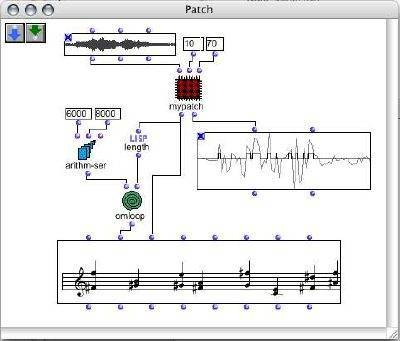
\includegraphics[width=0.8\textwidth]{openmusic.jpg}\\[1cm]
\caption{OpenMusic}
\label{OpenMusic}
\end{figure}

\par
Dans ce logiciel, les morceaux de musique sont constitués d'une suite d'arbres rythmiques. Comme décrit dans l'article \cite{agon}, \enquote{un arbre rythmique est défini comme un couple (D S) où D est une fraction (< 0) et S est une liste de n-éléments définissant n-proportions de D. Chaque élément de S peut-être soit un entier, soit un arbre rythmique.}

\par
Les images suivantes sont des exemples d'arbres rythmiques, en haut, et la partition correspondante, en bas.


\begin{minipage}[c]{.46\linewidth}
  \centering
  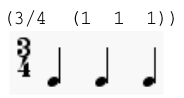
\includegraphics[width=0.5\textwidth]{rt1.png}\\[1cm]
\end{minipage}
\hfill
\begin{minipage}[c]{.46\linewidth}
  \centering
  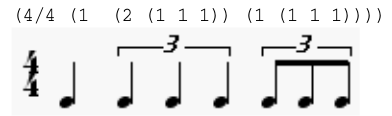
\includegraphics[width=0.9\textwidth]{rt2.png}\\[1cm]
\end{minipage}



\subsection{Le langage Java}

\par 
Java est un langage de programmation \textbf{orienté objet} fortement typé développé par \textbf{Sun Microsystems} à partir de \textbf{1995}. La société sera plus tard rachetée par \textbf{Oracle} en 2009 qui possède et maintient Java encore aujourd'hui.

\par 
Java se détache de la masse des autres langages de programmation notamment grâce à sa portabilité et sa facilité d'utilisation.

\begin{lstlisting}[caption=Hello world en java]
public class HelloWorld {
    public static void main(String[] args) {
        System.out.println("Hello world!");
    }
}
\end{lstlisting}

\par
Ci-dessus, un classique "Hello world" en Java. Nous pouvons y voir la définition de la classe \emph{HelloWorld} ainsi que la méthode principale du programme nommé \emph{main} et enfin un affichage sur la sortie standard.



\subsection{Le format MusicXML}

MusicXML \cite{musicxml} est un format de fichier permettant de représenter la notation musicale occidentale (notation classique, accords en notation anglo-saxonne, tablatures et percussions) et basé sur le langage XML. Il est propriétaire mais il peut librement utilisé avec une licence publique.

\par
Il y a plus de 20 ans, le format MIDI était très utilisé. Cependant, il n’est pas très adapté pour représenter toutes les caractéristiques de la musique, on perd donc en informations avec ce format. Pour pallier à cela, les formats SMDL et NIFF ont été créés. Cependant, le format SMDL était complexe et donc peu compréhensible. Il était donc très peu utilisé. Le format NIFF était un format peu pratique à utiliser et n’a donc pas été adopté par certains logiciels. Ces formats n’ont donc pas eu le succès souhaité.

\par
En 2004, la société Recordare LLC s’inspire des 2 formats universitaires MuseData et Humdrum pour créer la première version du format MusicXML. Ses avantages sont qu’il est facile à manipuler. Il permet le transfert de morceaux de musique d’une application à une autre. Il peut représenter beaucoup de caractéristiques de la musique. Cependant, il est verbeux, puisqu'il utilise le format XML, et ne donc permet pas de représenter la musique non occidentale.

\par
Il est de plus en plus utilisé puisque plus de 200 logiciels de musique l’ont adopté. Il est donc possible de travailler finement sur un morceau de musique en utilisant différents programmes.

\par
Comme le format XML est verbeux, le fichier prend de la place. La version 2.0, sortie en 2007, apporte donc la compression du fichier au format xml en un fichier au format mxl, et permet de diviser sa taille de façon importante. La version 3.0, sortie en 2011, permet le support des instruments virtuels.\\~\\

\par
On voit, dans le code correspondant à la partition suivante, que les informations sur la partition sont placées dans la balise "measure" et celle concernant la ronde sont contenues dans la balise "note".

\begin{figure}[!h] %h : here
\centering
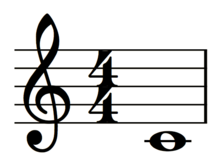
\includegraphics[width=0.2\textwidth]{musicxml_hello_world.png}\\[1cm]
%source : https://en.wikipedia.org/wiki/MusicXML
\caption{Hello World en MusicXML}
\label{Hello World en MusicXML}
\end{figure}


\begin{lstlisting}[caption=Document XML d'un Hello World en MusicXML, label=ruleml]
<?xml version="1.0" encoding="UTF-8" standalone="no"?>
<!DOCTYPE score-partwise PUBLIC
    "-//Recordare//DTD MusicXML 3.0 Partwise//EN"
    "http://www.musicxml.org/dtds/partwise.dtd">
<score-partwise version="3.0">
  <part-list>
    <score-part id="P1">
      <part-name>Music</part-name>
    </score-part>
  </part-list>
  <part id="P1">
    <measure number="1">
      <attributes>
        <divisions>1</divisions>
        <key>
          <fifths>0</fifths>
        </key>
        <time>
          <beats>4</beats>
          <beat-type>4</beat-type>
        </time>
        <clef>
          <sign>G</sign>
          <line>2</line>
        </clef>
      </attributes>
      <note>
        <pitch>
          <step>C</step>
          <octave>4</octave>
        </pitch>
        <duration>4</duration>
        <type>whole</type>
      </note>
    </measure>
  </part>
</score-partwise>
\end{lstlisting}



\subsection{Le langage XML}

Le langage XML \cite{xml_w3c, xml_ocr}, acronyme de e\textbf{X}tensible \textbf{M}arkup \textbf{L}angage, est langage de balisage générique spécifié par le W3C. Il permet de définir différents espaces de noms, c'est à dire des langages avec leur propre grammaire et vocabulaire. Il permet l'échange d'information entre des programmes très différents à condition d'utiliser la même grammaire.

\par
Il a l'avantage de pouvoir être compris par les êtres humains et les machines. Cependant, c'est un langage verbeux et qui peut donc prendre beaucoup de place s'il contient beaucoup d'information.

\par
Un document XML est constitué de balises pouvant contenir d'autres balises ou une valeur simple. Une balise peut aussi contenir des attributs donnant des informations supplémentaires sur le contenu.

\begin{lstlisting}[caption=Exemple d'un document XML]
<?xml version="1.0" encoding="UTF-8"?>
<racine>
    <balise attribut="valeur" >Contenu</balise>
    <baliseunique />
</racine>
\end{lstlisting}

\par
Ci-dessus un exemple de XML simpliste mais qui met en avant les bases du langage. La première ligne annonce le type de document et la version dans lequel le document va être rédigé. \emph{<racine>} est le nœud racine du document, celui qui en somme va contenir tout le document. On peut ici, facilement remarquer que le document peut être représenté sous la forme d'un arbre.

\par
XML permet à l'utilisateur de définir lui même la grammaire de son document grâce notamment aux \textbf{DTD} et au \textbf{Schéma XML}. Ces outils nous permettent de disposer de format d’échange de données tel que \textbf{MusicXML}.


\subsection{Le langage Relax NG}

\textbf{Relax NG} (\textbf{Re}gular \textbf{La}nguage for \textbf{X}ML \textbf{N}ext \textbf{G}eneration) née de la fusion de TreX de James Clark et de Relax de Murata Makoto. C'est un langage qui permet de définir la grammaire d'un document XML. Relax NG ne s'intéresse qu'à la structure du document et non à sa valeur.

\par
C'est ce que nous utiliserons afin de s'assurer de la validité du document à traiter.


\subsection{Affichage d'un graphe avec GraphStream}

Une fois le fichier XML parsé, nous disposons d'un \emph{DOM} sous forme d'un objet \emph{document}. Nous pouvons ensuite afficher l'arbre grâce à la librairie GraphStream \cite{graphstream}. Pour cela nous appelons un méthode qui affiche un nœud de l'arbre sur la racine du \emph{Document}. Cela nous permet donc d'afficher tout l'arbre.


\subsection{Les librairies}

Dans cette section, nous aborderons les librairies utilisées pour réaliser ce projet. Cela ira de la validation du XML en passant par le parsing de ce dernier, jusqu'à la récupération des information stockées dans le fichier MusicXML.


\subsubsection{Trang et Jing}

\textbf{Trang} \cite{trang} et \textbf{Jing} \cite{jing} sont deux librairies développées par \textbf{Thai Open Source}. Elles permettant de générer des grammaires Relax NG et de valider des documents XML à partir de cette même grammaire.

\par
Trang est une librairie qui permet de traduire un fichier de description grammaticale en fichier Relax NG. En effet XML n'est pas facilement lisible pour un esprit humain, c'est pour cela que Trang nous permet de créer notre grammaire dans un langage plus compréhensible. Une fois la grammaire écrite dans un fichier en \emph{.rnc}, nous pouvons générer notre fichier Relax NG en \emph{.rng}.

\par
Jing, quant à lui, est une librairie Java qui permet de valider un document XML à l'aide d'un fichier Relax NG.


\begin{lstlisting}[caption=Code java permettant de vérifier la validation d'un document XML]

final ValidationDriver vd = new ValidationDriver();
vd.loadSchema(rngFile);

if (!vd.validate(inputTextStream)) {
	throw new ParseException("Invalid xml :(");
} else {
    System.out.println("Valid xml :)");
}
\end{lstlisting}

\par
Le code ci-dessus est une utilisation simplifiée de Jing. Nous commençons tout d'abord par créer un objet \emph{ValidationDriver} de Jing dans lequel nous chargeons notre fichier Relax NG. Nous n'avons ensuite plus qu'à lancer la méthode \emph{validate(InputSource in) : boolean} qui nous indiquera si le document est valide.


\subsubsection{L'API SAX}

SAX \cite{sax_website, sax_oracle} est une API créée par David Megginson en 1998 et est l'acronyme de \textbf{S}imple \textbf{A}PI for \textbf{X}ML. Elle permet de manipuler des documents XML en utilisant des événements envoyées à chaque rencontre d'un élément.


\subsubsection{Le DOM}

Le DOM \cite{dom_w3c} , ou \textbf{D}ocument \textbf{O}bject \textbf{M}odel, est une interface de programmation normalisée par le W3C et est indépendant de tout plateforme et langage. Il voit les documents à balises comme des arbres dont le contenu et la structure peuvent être accédés et mis à jour dynamiquement.

\par
La figure suivante montre un exemple de DOM.

\begin{figure}[!h]
\centering
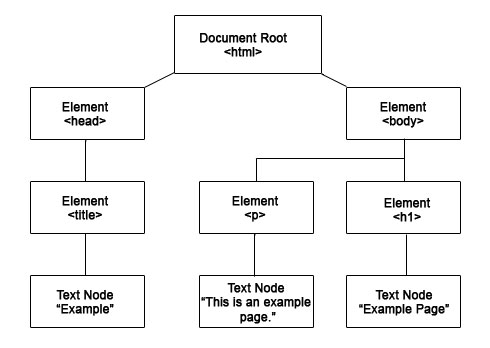
\includegraphics[width=0.8\textwidth]{ex_dom.jpg}\\[1cm]
%source : http://www.computerhope.com/jargon/d/dom.htm
\caption{Exemple d'un DOM}
\label{Exemple d'un DOM}
\end{figure}


\section{Architecture du programme}

\par
Dans cette section nous aborderons l'architecture du programme. C'est-à-dire la façon dont est organisé notre code et notamment les choix d’implémentation que nous avons effectués. Pour rappel, notre objectif est de générer un arbre rythmique et de récupérer la liste des accords et symboles musicaux pour réaliser l'affichage de la partition musical.

\subsection{Analyse du problème}

\par
Le format \emph{MusicXML} et plus généralement une partition musicale peut comporter énormement de symboles différents. C'est pour cela que nous avons du nous adapter à la structure très "personnalisable" et penser le code pour qu'il soit très malléable. Pour ce faire nous avons garder un niveau d'abstraction assez élevé pour pouvoir implémenter chaque symbole en modifiant le minimum de code. Lors de la réflexion qui a decoulé de ce constat, nous avons pu observer deux types de symbole : les symboles unaires et les symboles binaires.
\par
Les symboles unaires sont assez simple à implémenté dans le sens ou il n'influence pour la plupart du temps qu'une seule note. Il nous suffit donc de les stocker dans la dite note.
\par
En ce qui concerne les symboles binaires l'implémentation est beaucoup plus contraignante. Certains symboles comme les groupes de croches ont des marqueurs de début, continuation et fin alors que d'autres comme les groupes de laison n'ont qu'un début et une fin. Cela nous oblige donc à faire du sur-mesure pour bon certains symboles.
\par
Il demeure cependant des symboles qui peuvent concerner une mesure comme la partition. La balise \emph{<metronome>} par exemple est renseigné dans la mesure de la même  façon qu'une note. Il faut donc inclure ces exceptions.


\subsection{Architecture générale}

\par
Le programme se divise en trois parties. La première étant le parser. Cette partie permet au programme de disposer d'un \emph{DOM} à partir d'un fichier MusicXML. La seconde partie est la représentation objet des données contenues dans le \emph{DOM}. Et enfin la troisième partie est l'arbre rythmique qui pourra être généré à partir de la représentation objet de la partition.

\subsection{Parsing du fichier MusicXML}

\par
La première étape est de parser le document afin d'extraire les informations qu'il contient. C'est là qu'interviennent les éléments contenus dans le package \emph{pstl.musicxml.parsing}. Nous avons décidé d'encapsuler le parser XML natif de Java dans une classe \emph{XMLParser}. Ce choix est motivé pour plusieurs raisons.

\par
Tout d'abord pour ne laisser apparent que les fonctions du parser de Java que nous allons réellement utiliser afin de limiter le risque que nous ou un utilisateur tiers fasse usage du parser d'une mauvaise façon. Nous avons aussi fait ce choix pour simplifier l'utilisation de la classe pour que la création du parser qu'elle encapsule se fasse de la même façon à chaque fois. Et enfin ce choix a été rendu nécessaire à cause de \emph{Relax NG}. En effet comme nous ne faisons appel ni aux fichiers \emph{DTD} ni aux fichiers \emph{XML Schema}, il nous faut effectuer un prétraitement pour éliminer les références aux \emph{DTD} du fichier à parser. Vous pourriez vous demander pourquoi ne pas simplement utiliser les \emph{DTD} pour valider le document ? La raison est simple, la plupart des fichiers font référence aux \emph{DTD} en ligne fournis par MusicXML. Or ces derniers n'autorisent que les navigateurs web à accéder à de tels fichiers. Les possibilités qui s'offraient à nous étaient les suivantes : se faire passer pour un navigateur en modifiant quelques variables d’environnement. Cela aurait eu pour désavantage tout d'abord de ne pas être très rapide, l'accès à aux \emph{DTD} par réseau n'est pas très rapide comparé à un accès local. Nous jugions d'autre part la méthode peu honnête. En effet si l'organisation derrière MusicXML ne permet pas cela pour des raisons que j'imagine financières (par cela j'entends le coût engendré par la maintenance des serveurs) il n'aurait pas été juste d'outrepasser leurs instructions. Et enfin le dernier choix non retenu était celui de faire appel à des \emph{DTD} stockées localement. Cette méthode a été écartée bien que conseillée dans la documentation du format MusicXML car elle impliquait des redirections d'URI ce qui aurait fortement complexifié la création du parser.


\par
C'est donc pour toutes ces raisons que nous avons choisi d'utiliser \emph{Relax NG}. De plus, les fichiers décrivant la grammaire de MusicXML sont disponibles en ligne et l'auteur, qui les a déposés sur un projet GitHub \cite{relaxng_for_musicxml}, a fait preuve d'une certaine exhaustivité lors de la rédaction de ces derniers.

\par
Ce parser nous permet de disposer d'un \emph{DOM} (qui a pour nom de classe \emph{Document} avec Java) qui pourra être parcouru plus tard. Le schéma suivant récapitule les étapes pour passer du document XML au DOM.


\begin{figure}[!h]
\centering
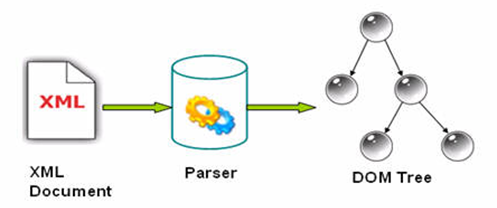
\includegraphics[width=0.5\textwidth]{parsing_xml_to_dom.png}\\[1cm]
%source : http://www.amfastech.com/2014/11/complete-tutorial-on-selecting-best-xml-parser.html
\caption{Parsing d'un document XML en DOM}
\label{Parsing d'un document XML en DOM}
\end{figure}


\subsection{Représentation objet de la partition}

\par
Nous aurions pu nous satisfaire du \emph{Document} retourné par le parser pour générer notre arbre rythmique mais cela aurait posé plusieurs problèmes. Tout d'abord la manipulation du \emph{DOM} n'est pas aisée. Cette structure de données basé sur des nœuds qui contiennent des fils, attributs et leur contenu textuel, doit être exploré d'une façon assez lourde à cause en partie du fait qu'un nœud n'est pas nativement un objet itérable comme les \emph{Collections} de Java par exemple. D'autre part, toutes les données contenues dans ces nœuds sont considérées comme des chaînes de caractère qui nécessitent un parsing et donc une manipulation assez verbeuse. De ce fait, il est plus simple pour nous de parcourir ce \emph{Document} une seule fois et d'extraire les données qu'il contient dans une structure de données plus aisément manipulable dans Java. Cela permet par exemple d'éviter des erreurs lors du développement des autres fonctionnalités de l'application qui se basent sur ces informations. Nous utilisons donc un ensemble de méthodes contenus dans la classe \emph{ScoreUtils} pour convertir notre \emph{Document} en instance de \emph{Score}.

\par
\emph{ScoreUtils} intègre aussi une partie très importante, la récupération des symboles contenus dans la partition. En effet, une partition n'est pas seulement un ensemble de notes il contient aussi un grand nombre de symbole ayant tous des significations très differentes pourvant aussi bien influancer la tonalité de la note ainsi que sa durée.

%Mettre des figures pour expliciter les partitions ? Un diagramme de class par exemple ?
%TODO établir un vrai package pour les partitions.

\par
La structure de données que nous avons élaborée se compose de la façon suivante : l'élément qui va contenir toutes les informations est la classe \emph{Score}. Une\emph{Score} contient une liste de \emph{Parts} qui l'on peut qualifier de \emph{Voix} en français. Chaque \emph{Part} contient un nom, un identifiant ainsi qu'une liste de \emph{Measures} (mesure) qui contient elle-même un numéro, une \emph{Signature}, une liste de \emph{IMusicalItem} et un \emph{Metronome} correspondant au tempo.

\part
\emph{IMusicalItem} est la super classe de bon nombre d'élément que nous pouvons qualifier de bout de chaine comme les \emph{Note}, \emph{Rest} (silence) ou encore les \emph{Tie} (liaison). Mais ce n'est pas tout, les groupes de \emph{IMusicalItem} sont également des \emph{IMusicalItem}. Cela nous permet entre autre de pouvoir imbriquer des groupes de \emph{IMusicalItem}. Dans les premières version de cette partie du code, il y n'y avait pas de lien entre les mesures et les groupes. Nous nous sommes rapidement rendu compte que la mesure et le groupe étaient à peu de chose près la même chose. Nous avons donc décidé qu'il serait mieux que le mesure soit aussi un groupe pour limiter la duplication de code. Un groupe peut représenter des croches liées ou encore un \emph{triolet}.

\par
Le tempo contient un type (une noire par exemple) et un nombre par minute. Ainsi, le tempo \emph{60 à la noire} signifie qu'il y a, dans une minute, 60 noires ou bien 30 blanches. Un élément musical possède aussi une liste de symboles musicaux. Un symbole musical représente une notation qui peut être une nuance comme un point ou encore un répétition par exemple.

\par
Pour chaque symbole musical, une classe lui est associée. Le symbole peut être unaire ou binaire. Les symboles unaires sont liés à une seule note, tel que les points d'orgues. Les symboles binaires sont liés à 2 notes, comme les liaisons. Pour chaque note, on récupère tous les symboles qui lui sont associés, on créé les objets intermédiaires et on les ajoute à l'objet \emph{Note}.

\par
La création de l'objet \emph{Score} se fait en deux étapes. Tout d'abord nous récuperons les données brutes dans le \emph{Document} que nous mettons dans l'objet \emph{Score} final. Une fois toutes ces données à disposition nous pouvons créer les groupes en fonction des symboles que nous rencontrons lors du parcours des mesures. Prenons comme exemple la balise \emph{<beam>} qui peut être présente dans une balise \emph{<note>} et qui contient les informations nécessaires pour représenter un groupe de croches dans \emph{MusicXML}. Cette balise a principalement un attribut \emph{number} qui designe le numéro du groupe actuel dans le cas où il a plusieurs groupes dans une mesure et qui contient l'énumeration suivante : \emph{begin, end, continue} qui nous permet de connaitre la position de la note dans le groupe. Lors de notre premier passage nous stockons ces informations dans un objet \emph{Beam}. Lors de notre second passage nous utilisons ces données pour créer nos groupes.
% TODO mettre ref à la doc de MusicXML ->
% http://usermanuals.musicxml.com/MusicXML/MusicXML.htm#EL-MusicXML-beam.htm%3FTocPath%3DMusicXML%2520Reference%7CScore%2520Schema%2520(XSD)%7CElements%7Cnote%7C_____18

\par
On pourrait penser que ce modèle de données est lourd, mais cela est largement compensé entre autres par l'aisance d'utilisation qu'il procure ainsi que la possibilité notamment de déduire les "coordonnées" des éléments qui le composent. En effet rien de plus facile que de dire qu'une note se trouve dans le \emph{Chord} 4 de la \emph{Measure} 2 de la \emph{Part} 2 de telle \emph{Score}. Ainsi nous pouvons par exemple utiliser ces coordonnées pour placer certains symboles à des endroits précis.


\subsection{Construction des arbres rythmiques}

Une fois la \emph{Score} créé, les arbres rythmiques pour chaque mesure sont construits. Cette étape est réalisée par les classes du package \emph{rhythmicstructures}. La classe factory \emph{RhythmicTreeFactory} parcours tout l'arbre des objets intermédiaires, et pour chaque \emph{Measure} rencontrée, un nouvel objet de la classe \emph{RhythmicTree} est créé. Ce dernier contient une \emph{Signature}, une \emph{Fraction}, un \emph{ItemType}, une liste d'\emph{ExtraSymbols} et une liste de \emph{RhythmicTree} correspondant aux fils. La seule étape que nous pouvons qualifier d'épineuse ici est celle qui consiste à traiter les groupes. Si une mesure contient des groupes imbriquées il faut créer les arbre rythmiques correspondant et les remplir. L'algorithme est donc récurcif, manipulation d'arbre oblige. Ayant pris le module d'algorithmique avancé qui traitait entre autres de manipulation d'arbres au premier semestre, nous avons pu réaliser cette algorithme sans trop de soucis.


\subsection{Test du programme}

Afin de vérifier que notre programme fonctionne correctement, une base de test a été créée dans le dossier \emph{test-data}. Elle est constituée de nombreux fichiers tests au format MusicXML. Chaque fichier contient quelques notes avec un symbole musical (signe crescendo, staccato, etc.). Chaque classe associée à un symbole peut ainsi être testée. Une partition complète de Bach est également présente pour tester sur un grand nombre de mesure.

\section{Conclusion}

conclusion


%%%%%%%%%%%%%%%%%%%%%%%%%%%%%%%%%%%%%%%%%%%%%%%  Annexes  %%%%%%%%%%%%%%%%%%%%

%\appendix %

%\include{annexes}


%%%%%%%%%%%%%%%%%%%%%%%%%%%%%%%%%%%%%%%%%%%%%%%  Bibliographie  %%%%%%%%%%%%%%%%%%%%

\bibliographystyle{IEEEtran}
\bibliography{IEEEabrv,biblio}
\nocite{*}

\end{document}
